\documentclass[11pt,a4paper]{article}
\usepackage[top=3cm, bottom=3cm, left=2.5cm, right=2.2cm]{geometry} %geometry of page
\usepackage[hidelinks]{hyperref} %reference links
\usepackage{fancyhdr} %header and footer control
\usepackage{minted} %source code syntax highlighting
\usepackage{qrcode} %qrcode links
\usepackage{graphicx} %images
\usepackage{tikz}
\usepackage{subcaption} %sub-figures

\usepackage{parskip}

% Breadboard connection diagrams: a wire drawn through the centres of every
% hole that is connected together. All coordinates are fractions of the
% breadboard image, with (0,0) bottom left and (1,1) top right, so they hold
% whatever width the image is drawn at.
\tikzset{
    wire/.style={line width=.8mm},
}
% Geometry below was measured off breadboard.png by fitting the hole centres,
% not estimated by eye: row n sits at 0.92940 - (n-1)*0.030014 (30 rows, fit
% residual under half a pixel), and the hole radius is 0.0121 of the width.
%
% one numbered row: columns A-E are wired as one group, F-J as another.
% The wires overhang the end holes so each group reads as separate.
\newcommand{\rowwire}[1]{%
    \pgfmathsetmacro{\rowy}{0.92940 - (#1-1)*0.030014}%
    \draw[wire] (0.2109, \rowy) -- (0.4343, \rowy);
    \draw[wire] (0.5458, \rowy) -- (0.7692, \rowy);
}
% one power rail, connected all the way down the board -- its holes line up
% with rows 1 to 30. Takes the x-fraction of the column: 0.0835 and 0.1410 on
% the left, 0.8583 and 0.9155 on the right.
\newcommand{\railwire}[1]{%
    \draw[wire] (#1, 0.048) -- (#1, 0.941);
}

\linespread{1.3}
\emergencystretch 3em

% Set Header and Footer
\fancyhead{}
\fancyhead[L]{\textbf{Lab 2: External LED}}
\fancyhead[R]{max.champneys@sheffield.ac.uk}
\fancyfoot{}
\fancyfoot[L]{\thepage}
\fancyfoot[R]{MAC 233 Arduino Labs, School of MAC, University of Sheffield}

% Create Document
\begin{document}
\pagestyle{fancy}

\section*{Prerequisites}
This worksheet builds upon the Lab 1 worksheet. You will have needed to complete the Lab 1 worksheet before you can continue with this lab. Out of your Arduino pack, you will need: 1 Arduino, 1 breadboard, 1 LED, 1 $220\Omega$ resistor, and 1 jumper cable.

\section*{Objectives}
The objective of today's lab is to learn how to use an electronic breadboard to create a circuit and to control an external output on the Arduino.

We will be taking the scenario from the previous worksheet and changing it to communicate with an external LED. Whilst this may sound complex, we are able to use the code from the previous worksheet as a starting point; therefore, it is only one new line of code and changing three existing lines of code.

\section{Understanding a Breadboard}
An electronic breadboard is a useful tool to create quick circuits. It becomes particularly helpful in our use case, as we can place our Arduino within the breadboard without any further adapters.

A breadboard can be thought of as a collection of rows (1\textrightarrow $N$) and columns (A\textrightarrow J), as in Figure \ref{fig:breadboard-plain}. Each row is wired together into two groups, divided by the centre separator. The first group is the columns A\textrightarrow E, and the second group is columns F\textrightarrow J. Each row is numbered from 1\textrightarrow $N$. Any item plugged into a hole will be accessible from any other hole within that same row group. None of this wiring is visible on the board itself, so Figure \ref{fig:breadboard-all} draws it in: any two holes joined by a wire are connected together, and holes on different wires are not.

\begin{figure}[ht!]
    \begin{center}
        \begin{subfigure}[t]{.45\textwidth}
            \centering
            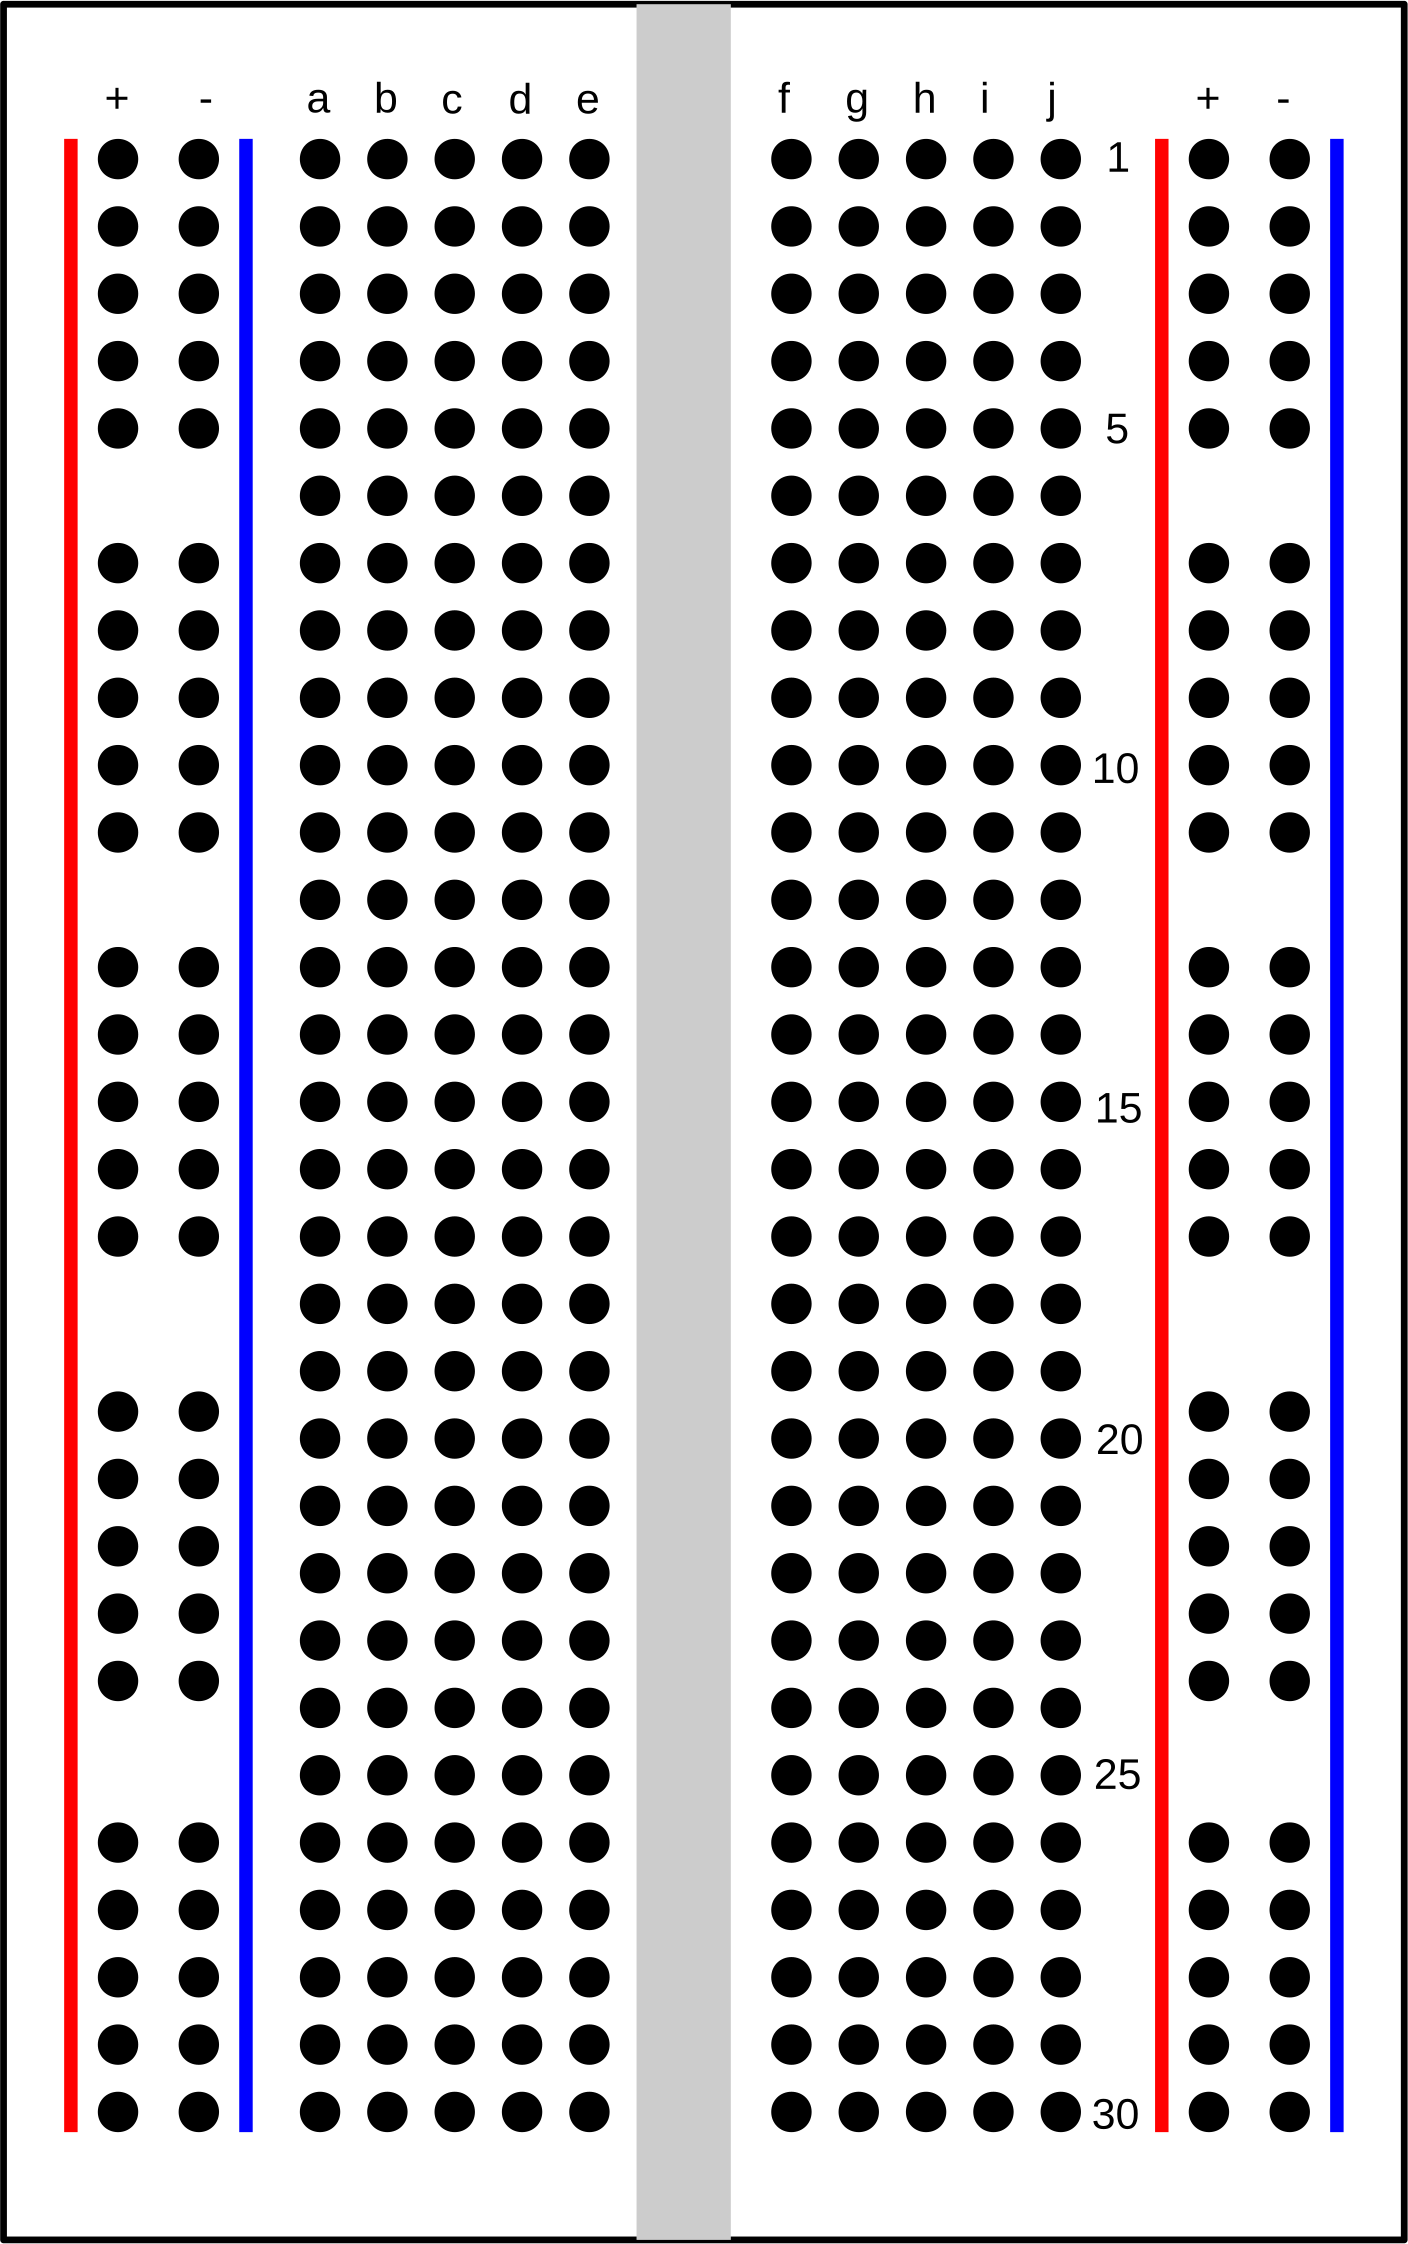
\includegraphics[width=\textwidth]{./images/breadboard.png}
            \caption{The board as you see it.}
            \label{fig:breadboard-plain}
        \end{subfigure}
        \hfill
        \begin{subfigure}[t]{.45\textwidth}
            \centering
            \begin{tikzpicture}
                %%breadboard
                \node[anchor=south west, inner sep=0] (bb) at (0, 0)
                    {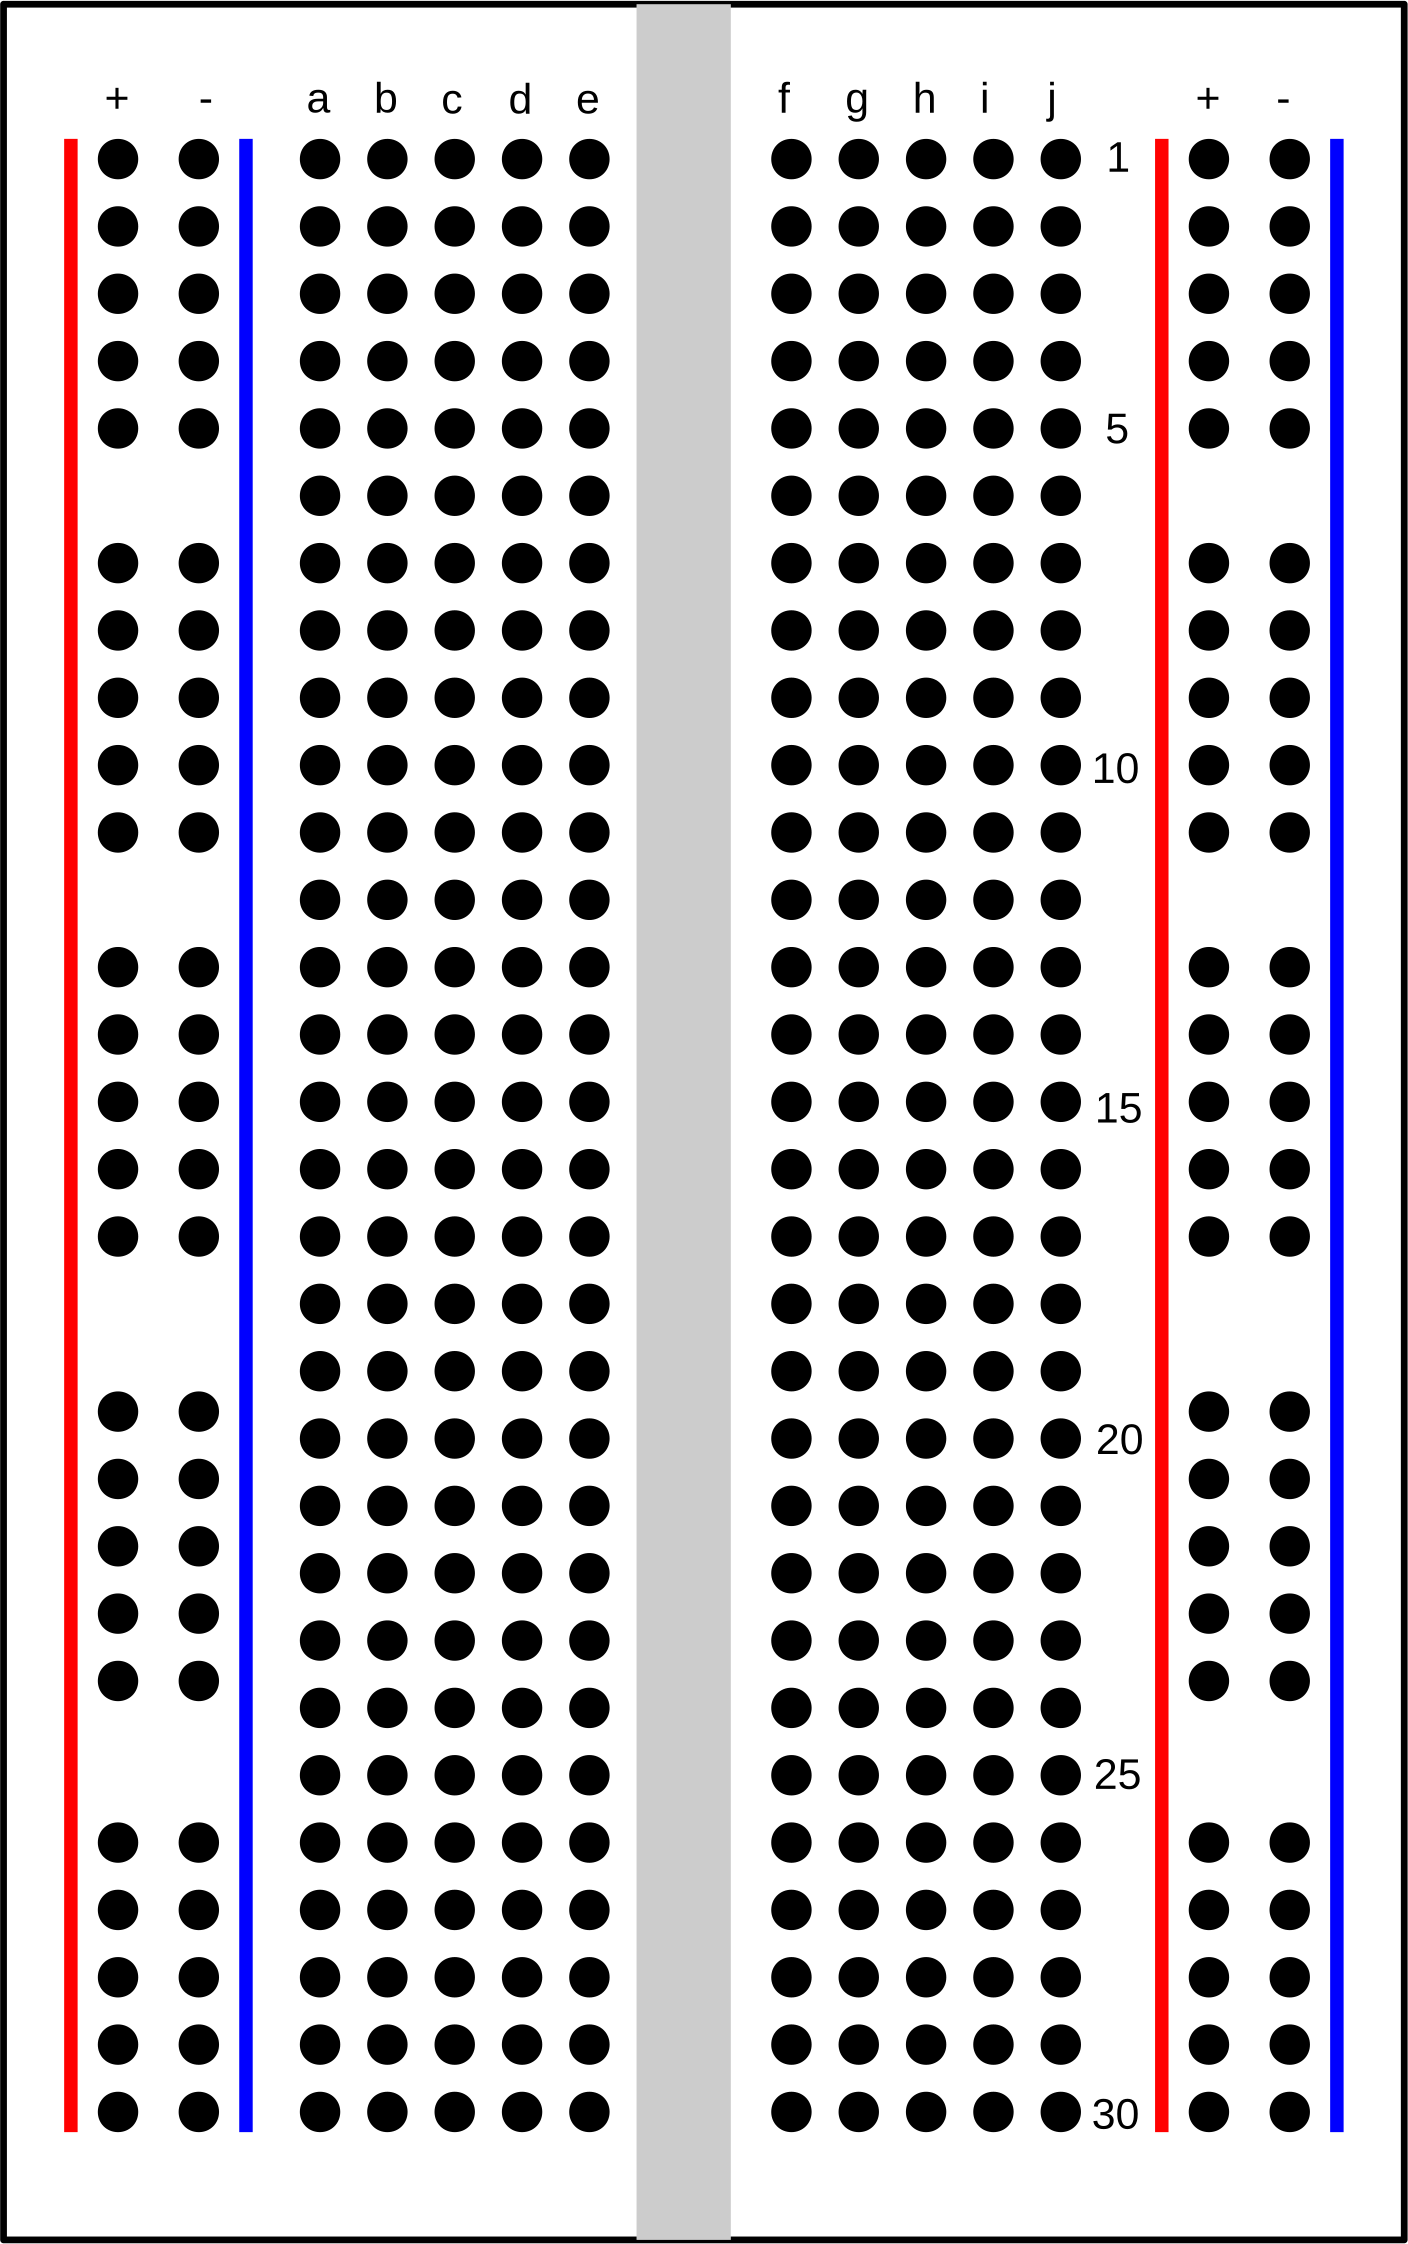
\includegraphics[width=\textwidth]{./images/breadboard.png}};
                \begin{scope}[x={(bb.south east)}, y={(bb.north west)}]
                    %% every numbered row
                    \foreach \r in {1,...,30}{ \rowwire{\r} }
                    %% all four power rails
                    \railwire{0.0835}
                    \railwire{0.1410}
                    \railwire{0.8583}
                    \railwire{0.9155}
                \end{scope}
            \end{tikzpicture}
            \caption{The same board with the hidden connections drawn in.}
            \label{fig:breadboard-all}
        \end{subfigure}\\
        \vspace{.5em}
        \scriptsize
        Original image source: \url{https://freesvg.org/breadboard}
    \end{center}
    \caption{An example electronic breadboard, showing which holes are wired together.}
\end{figure}

For instance, if you plugged the Arduino output for Pin D2 into column H on row 13, you would then be able to plug in an LED leg into column J on row 13. This would create a complete circuit so long as you have also completed the part of the circuit for the other LED leg.

There are also four power rails at either side of the breadboard, two on the left and two on the right. In our case these would carry +5V and GND, since that is what the Arduino Nano Every uses. All the holes in a rail's column are connected together: in Figure \ref{fig:breadboard-all} each rail is drawn as a single wire running the full length of the board.

\section{Creating the circuit}
The circuit needed for this worksheet is: Arduino Pin D2 \textrightarrow $220\Omega$ resistor \textrightarrow LED
\textrightarrow Arduino GND.

To do this, place your Arduino into the breadboard, such that the two rows of pins span the centre of the breadboard (this ensures we do not accidentally connect the pins to each other). Once this is done, use the Nano Every pinout diagram to find which pin on the Arduino is Pin D2: \url{https://docs.arduino.cc/resources/pinouts/ABX00028-full-pinout.pdf}. You then need to connect one leg of the $220\Omega$ resistor to Pin D2 of your Arduino through your breadboard. Then connect the other leg of the $220\Omega$ resistor to the positive leg of the LED (the longer leg). Finally, connect the negative leg of the LED to the ground pin on your Arduino through the jumper cable. You won't see anything visual happen at this stage; you need to write the code below into your sketch before the LED will light up.

\section{Changing the existing code}
Firstly, open your sketch from the previous worksheet into Arduino IDE. Once this is open, save the sketch under a new name (`File' \textrightarrow `Save As'). This will make sure you still have a copy of the sketch from Lab 1.

The first thing we are going to do is create a new definition for a \verb|LED_PIN| which will map to the Arduino Pin D2. To do this, copy the code below at the top of your file (before the Morse code definitions).

\inputminted[
    autogobble, stripnl,
    rangestartstring={\#define LED_PIN},
    rangestopbeforestring={/*},
]{arduino}{../lab-2-led.ino}

The internal LED on an Arduino is referenced in exactly the same way as you would reference an external pin. This means all we need to do is change anywhere within our code that uses \verb|LED_BUILTIN| to use the newly defined external pin \verb|LED_PIN|. This means changing the code to the following lines:

% not pulled from the sketch: these lines are scattered through setup and loop,
% and the comments are instructions to the student rather than sketch comments
\begin{minted}{arduino}
// this line is in the setup function
pinMode(LED_PIN, OUTPUT);

// these two lines are in the loop function
// note: there is a line of code between these two lines
digitalWrite(LED_PIN, HIGH);
digitalWrite(LED_PIN, LOW);
\end{minted}

\section{Try it out on your Arduino}
You now should be able to compile your sketch (`Sketch' \textrightarrow `Verify\textbackslash Compile') and then upload to your Arduino (`Sketch' \textrightarrow `Upload'). You should see that your Arduino now blinks the externally connected LED in the same pattern as it did on your internal LED.

If you have managed to get the external LED to turn on and off with the Morse code signal, see if you can change your code so that `dot' signals are displayed on the internal LED, and `dash' signals are displayed on the external LED.

For a final (harder) challenge, see if you can rewrite the code to show fully decodable Morse code. Real Morse code has rules about the length of the gaps between signals, between letters, and between words. The rules are set out on the Wikipedia page: \url{https://en.wikipedia.org/wiki/Morse_code}.

\pagebreak
\section*{Help}
If you are having issue compiling the project or don't understand where each section goes, you can see a complete version of the sketch with additional source code comments at \url{https://github.com/MDCHAMP/MAC233/blob/main/labs/lab-2-led/lab-2-led.ino}.

\vspace{2em}

\begin{center}
    \qrcode[hyperlink, height=6cm]{https://github.com/MDCHAMP/MAC233/blob/main/labs/lab-2-led/lab-2-led.ino}
\end{center}

\vspace{2em}

Additionally, if you are wondering how to wire up the circuit required for this lab on the breadboard, the electronic wiring diagram is below.

\begin{center}
    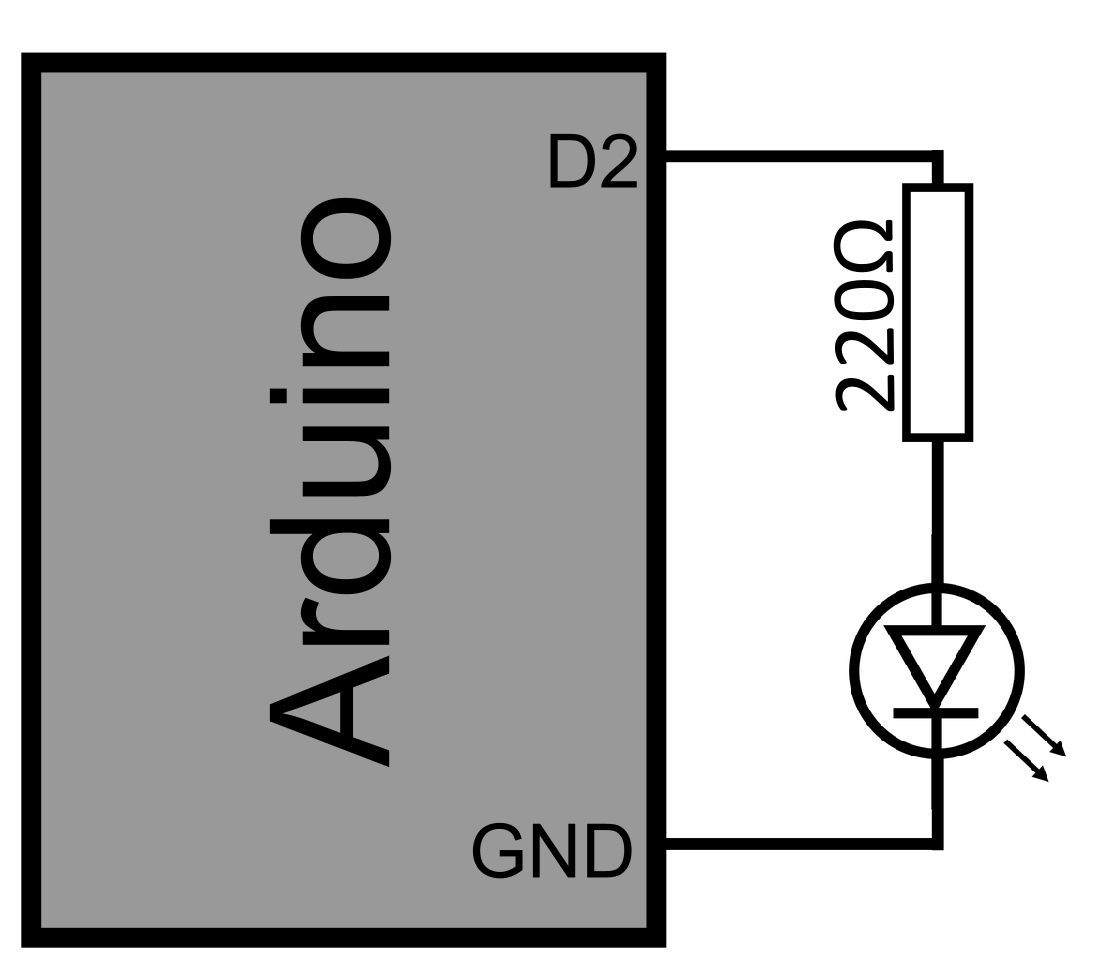
\includegraphics[width=.4\textwidth]{./images/wiring-diagram.png}
\end{center}

\end{document}